\section{Finaler Entwurf}
\subsection{Entwurfsziele}
Mit den vorgestellten Überlegungen soll versucht werden das Design endlich auf die erforderliche Größe zu schrumpfen.
Die Ausführungszeit sollte dabei nicht mehr als bereits in den Überlegungen beschrieben.

\subsection{Aufbau}
\begin{figure}
	\center
	\caption{Atomlayout des Beschleunigers}
	\label{fig:layout_iteration_3}
\end{figure}
\begin{figure}
	\center
	\includegraphics{images/iteration_3.pdf}
	\caption{Aufbau der A-Atome}
	\label{fig:aufbau_iteration_3}
\end{figure}
\begin{figure}
	\center
	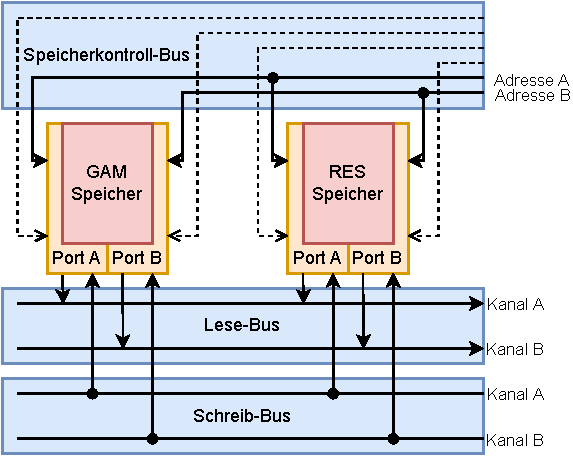
\includegraphics{images/Speicheranbindung.pdf}
	\caption{Speicheranbindung}
	\label{fig:speicheranbindung_iteration_3}
\end{figure}
Der Beschleuniger besteht diesmal aus insgesamt vier Atomen. Die beiden Atome A0 und A1 haben denselben Aufbau und sind für die eigentliche Berechnung der Permutationsfunktion zuständig.
Die Atome B0 und B1 lesen während der Berechnung schon den nächsten Datenblock aus dem externen Speicher ein und konvertieren ihn in Tiles, die dann von den A-Atomen entgegen genommen werden.
Der Beschleuniger besteht wie auch im vorherigen Entwurf aus zwei identischen Atomen, deren Funktionsweise über den Atom-Index definiert wird.
Da der Datenspeicher in den BRAM verschoben wird, müssen die anderen Komponenten so umgebaut werden, dass sie mit dem Interface des BRAM funktionieren.
Dafür werden alle Komponenten sowie der BRAM über einen Speicherbus miteinander verbunden (Abb. \ref{fig:aufbau_iteration_3}).

\subsubsection{BRAM}
Die beiden verwendeten BRAM-Bänke GAM (für Gamma) und RES (für Result) besitzen jeweils zwei Lese-Schreib-Ports, mit denen jeweils ein Tile-Block (bestehend aus zwei benachbarten Tiles) gelesen und auch gleichzeitig geschrieben werden kann (read before write).
Je ein Port ist dabei an den A-Kanal und der Andere an den B-Kanal angeschlossen. 

\subsubsection{Speicherbus}
Der Speicherbus besteht aus drei Segmenten (Abb. \ref{fig:speicheranbindung_iteration_3}). Auf dem Lese-Bus werden Daten aus dem BRAM ausgelesen und den anderen Modulen zur Verfügung gestellt.
Er besteht aus zwei Kanälen, die beide einen Tile-Block breit sind.
Auf dem Schreib-Bus werden Daten von den Berechnungsmodulen und dem Kommunikationsmodul gesammelt und an den BRAM weitergegeben.
Auch dieser besteht aus zwei ein-Tile-Block breiten Kanälen.
Über den Speicherkontroll-Bus werden alle Steuersignale für den BRAM gesammelt. Er besteht aus zwei 7 Bit breiten Address-Vektoren für die beiden Datenkanäle
sowie einem Read-Enable-Signal und einem Write-Enable-Signal für jeden der insgesamt vier Ports.

\subsubsection{Zustandsautomat}
Der Zustandsautomat besteht nicht mehr aus einer Einheit, sondern besteht nun aus einer zentralen Kontrolle sowie spezialisierten Kontrolleinheiten innerhalb der Berechnungseinheiten, angedeutet durch die lila Blöcke.
Die zentrale Kontrolleinheit steuert dabei nur noch den Betriebsmodus des Kommunikationsmoduls und stößt die Abarbeitung in den Berechnungseinheiten an.
Die Kontrolle innerhalb der Berechnungseinheiten bekommt bei Aktivierung die Kontrolle über den Speicherkontroll-Bus und generiert die Steuersignale für die Berechnungseinheit und den Speicher.
Ist die Abarbeitung einer Berechnungseinheit abgeschlossen, wird die Kontrolle wieder an die zentrale Kontrolleinheit übergeben.

\subsubsection{Kommunikationsmodul}
Das Kommunkationsmodul dient zum Datenaustausch zwischen den Atomen sowie zur Kommunikation mit dem externen Speicher, der die Eingabedaten bereitstellt und das Ergebnis entgegennimmt.
Für jede Berechnungseinheit gibt es einen Betriebsmodus, der festlegt, welche Daten von der Berechnungseinheit und dem Speicherbus ausgegeben werden und welche empfangenen Daten an den Speicherbus und die Berechnungseinheit
weitergegeben werden. Dieser Betriebsmodus wird von der zentralen Kontrolleinheit bestimmt.

\subsubsection{Gamma}
Das Gamma-Modul berechnet analog zum Modul aus dem vorherigen Entwurf immer zwei Slices und gibt die entsprechenden Tiles an den Speicher und über das Kommunikationsmodul an das andere Atom aus.
Bis auf die Einführung des Kontrollblocks und einer leichten Anpassung der Schnittstelle ist es identisch zum vorherigen Design. Es nimmt die Eingabedaten aus dem RES-Speicher und schreibt das Ergebnis in den GAM-Speicher

\subsubsection{Rho-Puffer}
\begin{figure}
	\center
	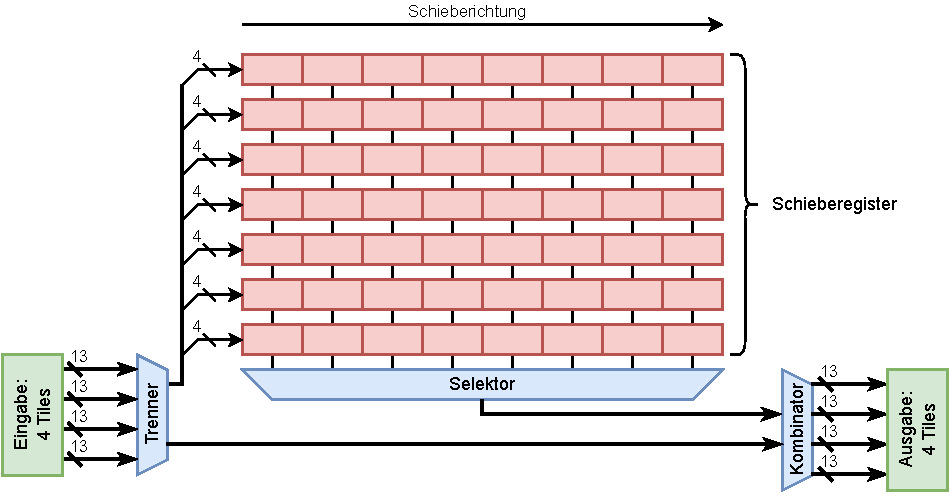
\includegraphics{images/Rho-Aufbau.pdf}
	\caption{Aufbau des Rho-Puffers}
	\label{fig:rho_aufbau_iteration_3}
\end{figure}
Der Rho-Puffer besteht aus sieben 32-Bit-Schieberegistern, die wie in [Ref] verwendet werden, um interativ die Bit-Rotationen zu berechnen (Abb. \ref{fig_rho_aufbau_iteration_3}).
Dazu wird die Berechnung in zwei Schritte unterteilt. Im ersten Schritt werden die Daten aus dem GAM-Speicher gelesen und auf den betrffenden Lanes wird eine Linksrotation durchgeführt, während die anderen Lanes unverändert bleiben.
Das Ergebnis wird im wieder im GAM-Speicher gespeichert. Im zweiten Schritt werden die Daten aus dem GAM-Speicher erneut ausgelesen und diesmal wird auf den übrigen Lanes eine Rechtsrotation durchgeführt. Das finale Ergebnis der Rho-Berechnung
wird dann im RES-Speicher wieder abgespeichert. Es ist die einzige Berechnungseinheit, die keinerlei Kommunikation benötigt und ist daher auch nicht an das Kommunikationsmodul angeschlossen.

\subsubsection{Einlesemodul}
Um das Ergebnis einer Permutation mit einem neuen Datenblock gemäß der Schwammkonstruktion zu kombinieren, müssen die eingelesenen Daten mit den Daten im Ergebnisspeicher mit einem XOR kombiniert werden.
Das Einlesemodul macht genau das und schreibt die kombinierten Daten wieder zurück in den Ergebnisspeicher, sodass erneut die Permutation berechnet werden kann.
Während die neuen Daten eingelesen werden, kann jedoch die eigentliche Berechnung nicht durchgeführt werden. Daher ist es wichtig, dass dieser Schritt so schnell wie möglich abläuft.
Dazu werden die Daten den Atomen direkt als Tiles bereitgestellt, sodass die Einleseeinheit nicht erst die Lanes in Tiles konvertieren muss. Da der Datenblock jedoch in Lanes gespeichert ist,
muss dieser Konvertierungsprozess bereits im Vorhinein irgendwo ausgeführt werden.
Diese Aufgabe übernehmen die Atome B0 und B1. Da die Berechnung der Permutation länger dauert als das Einlesen und die Konvertierung des Datenblocks aus dem externen Speicher,
hat dieser zusätzliche Schritt keinerlei Auswirkung auf die Berechnungsgeschwindigkeit.

\subsubsection{Ergebnismodul}
Zur Ausgabe des 256-Bit Hashes wird das Ergebnismodul verwendet. Es besteht aus einem in FFs implementierten Puffer, der mit den Daten des Ergebnisspeichers gefüllt wird und die Daten so zurück in Lanes konvertiert.
So kann das Ergebnis direkt im richtigen Format ausgegeben werden und im externen Speicher übernommen werden.

\subsection{Berechnung der Permutationsfunktion}
Da die Daten im BRAM nur Slice orientiert als Tiles gespeichert werden und die Eingabedaten aber als Lanes vorliegen, müssen sie erst konvertiert werden.
Diese Konvertierung findet während der vorherigen Berechnung in den B-Atomen statt.
Dabei lesen die B-Atome mehrfach den gesammten Datenblock und puffern immer einen Teil aller Lanes, bis sie sie als vollständige Tiles speichern können.
Dass dabei jede Lane mehrfach eingelesen werden muss, hat keinen Einfluss auf die Ausführunszeit des Beschleunigers, da die Berechnungszeit der modifizierten Rundenfunktion größer ist,
als die Berechnungszeit der Konvertierer und beide Systeme vollständig parallel arbeiten können.
Nachdem ein Block konvertiert wurde und die A-Atome bereit sind, werden die Tiles der Reihe nach über das Kommunikationsmodul von den B-Atomen zum Einlesemodul der A-Atome übertragen
und mit den Daten aus dem RES-Block über ein XOR kombiniert und anschließend wieder in den RES-Block übernommen.
Für die Gamma-Berechnung werden die Slices über den Lesebus aus dem RES-Block gelesen an die Recheneinheit sowie an die Kommunikationseiheit übergeben.
Die Ergebnisse werden anschließend vom Kommunikationsmodul und der Recheneinheit über den Schreib-Bus in den GAM-Block geschrieben.
Anschließend wird die Links-Rotation mit Hilfe des Rho-Puffers durchgeführt. Die Daten werden aus dem GAM-Block über den Datenbus an den Puffer übertragen.
Zuerst wird der Puffer mit den Initialdaten gefüllt, dann werden wie im Abschnitt [Ref] die Tiles nach und nach in den Puffer eingeschoben
und die Erbebnis-Tiles werden über den Schreib-Bus wieder in den GAM-Block übernommen.
Die Rechts-Rotation wird genau so durchgeführt, nur werden dieses Mal die Ergebnisse in den RES-Block geschrieben anstatt in den GAM-Block.
Hier wird auch ein Vorteil des Bus-Designs deutlich: Da beide Blöcke ihre Daten über den Bus empfangen, braucht für die Rechts-Rotation nur das
Write-Enable-Signal verändert werden und die Ergebnisse müssen nicht auf eine andere Eingabe umgeleitet werden.
Die Rho und Gamma Funktionen werden so oft abwechselnd berechnet, bis der Block gemäß der KECCAK-P Funktion verarbeitet wurde.
Danach kann über den Kontrollvektor bestimmt werden, ob entweder der nächste Block eingelesen werden, oder das Ergenis ausgegeben werden soll.
Für die Ausgabe des Ergebnisses werden alle 64 Tiles im Atom A0 vom Ergebnismodul ausgelesen und die ersten 4 Bits in einem FF-Puffer gespeichert.
Als letztes werden diese Ergebnisbits als Lanes ausgegeben und im externen Speicher als Endergebnis gespeichert.

\subsection{Bewertung}

\subsection{Weitere Optimierungsansätze}

\subsubsection{Auslagerung der Ergebniskonvertierung}
Das Ergebnismodul nimmt unnötig viel Platz im Atom ein und ist eigentlich nur deshalb in den A-Atomen enthalten, weil der Platz nicht weiter benötigt wird.
Es lässt sich aber auch in die B-Atome verschieben, die auch die Konvertierung für die Eingabe übernehmen auf Kosten eines weiteren Kommunikationsschrittes.
So kann noch ein wenig Platz für weitere Optimierungen geschaffen werden, die mit ein wenig mehr Platz die Berechnungsgeschwindigkeit wieder verbessern.

\subsubsection{Reduktion auf 1 Atom}
Die Berechnung wurde ursprünglich auf zwei Atome aufgeteilt, damit die Datenmenge reduziert werden kann, die ein Atom halten muss.
Durch die Einführung des BRAM fällt diese Optimierung weg, da der BRAM mehr als genug Platz bereitstellt.

\subsubsection{Erweiterung des Speicherinterfaces auf mehr Tiles}
Die Aufteilung des Speichers in zum Beispiel 4 Tiles erlaubt es eine größere Menge an Tiles gleichzeitig für die Berechnung von Rho bereit zu stellen.
Da in einem zwei Atom Ansatz die Gamma-Funktion durch die Bandbreite des Datenkanals begrenzt ist, würde dieser Teil keine Beschleunigung erfahren.
In einem Ein-Atom-Ansatz hingegen würden allerdings auch hier noch mehr Slices gleichzeitig berechnet werden können.

\subsubsection{Erweiterung des Rho-Puffers}
Durch 1 Atom Ansatz müssen alle Lanes in einem Atom berechnet werden, kann der Puffer erweitert werden oder braucht das zu viel Platz?
Müssen mehr als 2 Rotationen durchgeführt werden?

\subsubsection{Auslagerung der Rho-Berechnung}
Auch wenn alle Daten in einem Atom gespeichert werden, könnte es sinnvoll sein, die Berechnung von Rho auf verschiedene Atome zu verteilen.
[Schaubild]. So können beim Filtern der Lanes die restlichen Lanes an ein anderes Atom übertragen werden, das die Rotation durchführt.
So kann die Größenbeschränkung des Puffers umgangen werden. Wird auch dieser Prozess durch eine Pipeline realisiert, beträgt die maximale Bandbreite hierfür
max k s.t. k * 7 <= 32
=> k = 4 Slices. Wird der Puffer im Hauptatom noch ein wenig erweitert, sodass maximal 6 Lanes gleichzeitig ausgelagert werden müssen, so steigt die Bandbreite sogar
auf 5 Slices. Da allerdings immer zwei Ports für die Zusammensetzung der Daten verantwortlich sind, müssten immer 6 Slices gleichzeitig gelesen werden und die
Restlichen in einem weiteren Puffer zwischengehalten werden was die Komplexität weiter erhöht. Außerdem ist ein solcher Ansatz nicht mehr symmetisch,
heißt es kann nicht der gleiche Beschleuniger auf beide Atome geladen werden.

\subsubsection{Erhöhung der Berechnungsfrequenz (Nutzung der fallenden Taktflanken)}